\chapter{plotting methods}
\begin{figure}[]
    \begin{center}
        \fbox{\scalebox{0.5}{%% Creator: Matplotlib, PGF backend
%%
%% To include the figure in your LaTeX document, write
%%   \input{<filename>.pgf}
%%
%% Make sure the required packages are loaded in your preamble
%%   \usepackage{pgf}
%%
%% Also ensure that all the required font packages are loaded; for instance,
%% the lmodern package is sometimes necessary when using math font.
%%   \usepackage{lmodern}
%%
%% Figures using additional raster images can only be included by \input if
%% they are in the same directory as the main LaTeX file. For loading figures
%% from other directories you can use the `import` package
%%   \usepackage{import}
%%
%% and then include the figures with
%%   \import{<path to file>}{<filename>.pgf}
%%
%% Matplotlib used the following preamble
%%
\begingroup%
\makeatletter%
\begin{pgfpicture}%
\pgfpathrectangle{\pgfpointorigin}{\pgfqpoint{6.400000in}{4.800000in}}%
\pgfusepath{use as bounding box, clip}%
\begin{pgfscope}%
\pgfsetbuttcap%
\pgfsetmiterjoin%
\definecolor{currentfill}{rgb}{1.000000,1.000000,1.000000}%
\pgfsetfillcolor{currentfill}%
\pgfsetlinewidth{0.000000pt}%
\definecolor{currentstroke}{rgb}{1.000000,1.000000,1.000000}%
\pgfsetstrokecolor{currentstroke}%
\pgfsetdash{}{0pt}%
\pgfpathmoveto{\pgfqpoint{0.000000in}{0.000000in}}%
\pgfpathlineto{\pgfqpoint{6.400000in}{0.000000in}}%
\pgfpathlineto{\pgfqpoint{6.400000in}{4.800000in}}%
\pgfpathlineto{\pgfqpoint{0.000000in}{4.800000in}}%
\pgfpathlineto{\pgfqpoint{0.000000in}{0.000000in}}%
\pgfpathclose%
\pgfusepath{fill}%
\end{pgfscope}%
\begin{pgfscope}%
\pgfsetbuttcap%
\pgfsetmiterjoin%
\definecolor{currentfill}{rgb}{1.000000,1.000000,1.000000}%
\pgfsetfillcolor{currentfill}%
\pgfsetlinewidth{0.000000pt}%
\definecolor{currentstroke}{rgb}{0.000000,0.000000,0.000000}%
\pgfsetstrokecolor{currentstroke}%
\pgfsetstrokeopacity{0.000000}%
\pgfsetdash{}{0pt}%
\pgfpathmoveto{\pgfqpoint{0.800000in}{0.960000in}}%
\pgfpathlineto{\pgfqpoint{5.760000in}{0.960000in}}%
\pgfpathlineto{\pgfqpoint{5.760000in}{4.224000in}}%
\pgfpathlineto{\pgfqpoint{0.800000in}{4.224000in}}%
\pgfpathlineto{\pgfqpoint{0.800000in}{0.960000in}}%
\pgfpathclose%
\pgfusepath{fill}%
\end{pgfscope}%
\begin{pgfscope}%
\pgfsetbuttcap%
\pgfsetroundjoin%
\definecolor{currentfill}{rgb}{0.000000,0.000000,0.000000}%
\pgfsetfillcolor{currentfill}%
\pgfsetlinewidth{0.803000pt}%
\definecolor{currentstroke}{rgb}{0.000000,0.000000,0.000000}%
\pgfsetstrokecolor{currentstroke}%
\pgfsetdash{}{0pt}%
\pgfsys@defobject{currentmarker}{\pgfqpoint{0.000000in}{-0.048611in}}{\pgfqpoint{0.000000in}{0.000000in}}{%
\pgfpathmoveto{\pgfqpoint{0.000000in}{0.000000in}}%
\pgfpathlineto{\pgfqpoint{0.000000in}{-0.048611in}}%
\pgfusepath{stroke,fill}%
}%
\begin{pgfscope}%
\pgfsys@transformshift{0.899200in}{0.960000in}%
\pgfsys@useobject{currentmarker}{}%
\end{pgfscope}%
\end{pgfscope}%
\begin{pgfscope}%
\definecolor{textcolor}{rgb}{0.000000,0.000000,0.000000}%
\pgfsetstrokecolor{textcolor}%
\pgfsetfillcolor{textcolor}%
\pgftext[x=0.825556in, y=0.744527in, left, base,rotate=30.000000]{\color{textcolor}\rmfamily\fontsize{10.000000}{12.000000}\selectfont \(\displaystyle {0}\)}%
\end{pgfscope}%
\begin{pgfscope}%
\pgfsetbuttcap%
\pgfsetroundjoin%
\definecolor{currentfill}{rgb}{0.000000,0.000000,0.000000}%
\pgfsetfillcolor{currentfill}%
\pgfsetlinewidth{0.803000pt}%
\definecolor{currentstroke}{rgb}{0.000000,0.000000,0.000000}%
\pgfsetstrokecolor{currentstroke}%
\pgfsetdash{}{0pt}%
\pgfsys@defobject{currentmarker}{\pgfqpoint{0.000000in}{-0.048611in}}{\pgfqpoint{0.000000in}{0.000000in}}{%
\pgfpathmoveto{\pgfqpoint{0.000000in}{0.000000in}}%
\pgfpathlineto{\pgfqpoint{0.000000in}{-0.048611in}}%
\pgfusepath{stroke,fill}%
}%
\begin{pgfscope}%
\pgfsys@transformshift{1.801018in}{0.960000in}%
\pgfsys@useobject{currentmarker}{}%
\end{pgfscope}%
\end{pgfscope}%
\begin{pgfscope}%
\definecolor{textcolor}{rgb}{0.000000,0.000000,0.000000}%
\pgfsetstrokecolor{textcolor}%
\pgfsetfillcolor{textcolor}%
\pgftext[x=1.667233in, y=0.709804in, left, base,rotate=30.000000]{\color{textcolor}\rmfamily\fontsize{10.000000}{12.000000}\selectfont \(\displaystyle {50}\)}%
\end{pgfscope}%
\begin{pgfscope}%
\pgfsetbuttcap%
\pgfsetroundjoin%
\definecolor{currentfill}{rgb}{0.000000,0.000000,0.000000}%
\pgfsetfillcolor{currentfill}%
\pgfsetlinewidth{0.803000pt}%
\definecolor{currentstroke}{rgb}{0.000000,0.000000,0.000000}%
\pgfsetstrokecolor{currentstroke}%
\pgfsetdash{}{0pt}%
\pgfsys@defobject{currentmarker}{\pgfqpoint{0.000000in}{-0.048611in}}{\pgfqpoint{0.000000in}{0.000000in}}{%
\pgfpathmoveto{\pgfqpoint{0.000000in}{0.000000in}}%
\pgfpathlineto{\pgfqpoint{0.000000in}{-0.048611in}}%
\pgfusepath{stroke,fill}%
}%
\begin{pgfscope}%
\pgfsys@transformshift{2.702836in}{0.960000in}%
\pgfsys@useobject{currentmarker}{}%
\end{pgfscope}%
\end{pgfscope}%
\begin{pgfscope}%
\definecolor{textcolor}{rgb}{0.000000,0.000000,0.000000}%
\pgfsetstrokecolor{textcolor}%
\pgfsetfillcolor{textcolor}%
\pgftext[x=2.508911in, y=0.675082in, left, base,rotate=30.000000]{\color{textcolor}\rmfamily\fontsize{10.000000}{12.000000}\selectfont \(\displaystyle {100}\)}%
\end{pgfscope}%
\begin{pgfscope}%
\pgfsetbuttcap%
\pgfsetroundjoin%
\definecolor{currentfill}{rgb}{0.000000,0.000000,0.000000}%
\pgfsetfillcolor{currentfill}%
\pgfsetlinewidth{0.803000pt}%
\definecolor{currentstroke}{rgb}{0.000000,0.000000,0.000000}%
\pgfsetstrokecolor{currentstroke}%
\pgfsetdash{}{0pt}%
\pgfsys@defobject{currentmarker}{\pgfqpoint{0.000000in}{-0.048611in}}{\pgfqpoint{0.000000in}{0.000000in}}{%
\pgfpathmoveto{\pgfqpoint{0.000000in}{0.000000in}}%
\pgfpathlineto{\pgfqpoint{0.000000in}{-0.048611in}}%
\pgfusepath{stroke,fill}%
}%
\begin{pgfscope}%
\pgfsys@transformshift{3.604655in}{0.960000in}%
\pgfsys@useobject{currentmarker}{}%
\end{pgfscope}%
\end{pgfscope}%
\begin{pgfscope}%
\definecolor{textcolor}{rgb}{0.000000,0.000000,0.000000}%
\pgfsetstrokecolor{textcolor}%
\pgfsetfillcolor{textcolor}%
\pgftext[x=3.410729in, y=0.675082in, left, base,rotate=30.000000]{\color{textcolor}\rmfamily\fontsize{10.000000}{12.000000}\selectfont \(\displaystyle {150}\)}%
\end{pgfscope}%
\begin{pgfscope}%
\pgfsetbuttcap%
\pgfsetroundjoin%
\definecolor{currentfill}{rgb}{0.000000,0.000000,0.000000}%
\pgfsetfillcolor{currentfill}%
\pgfsetlinewidth{0.803000pt}%
\definecolor{currentstroke}{rgb}{0.000000,0.000000,0.000000}%
\pgfsetstrokecolor{currentstroke}%
\pgfsetdash{}{0pt}%
\pgfsys@defobject{currentmarker}{\pgfqpoint{0.000000in}{-0.048611in}}{\pgfqpoint{0.000000in}{0.000000in}}{%
\pgfpathmoveto{\pgfqpoint{0.000000in}{0.000000in}}%
\pgfpathlineto{\pgfqpoint{0.000000in}{-0.048611in}}%
\pgfusepath{stroke,fill}%
}%
\begin{pgfscope}%
\pgfsys@transformshift{4.506473in}{0.960000in}%
\pgfsys@useobject{currentmarker}{}%
\end{pgfscope}%
\end{pgfscope}%
\begin{pgfscope}%
\definecolor{textcolor}{rgb}{0.000000,0.000000,0.000000}%
\pgfsetstrokecolor{textcolor}%
\pgfsetfillcolor{textcolor}%
\pgftext[x=4.312547in, y=0.675082in, left, base,rotate=30.000000]{\color{textcolor}\rmfamily\fontsize{10.000000}{12.000000}\selectfont \(\displaystyle {200}\)}%
\end{pgfscope}%
\begin{pgfscope}%
\pgfsetbuttcap%
\pgfsetroundjoin%
\definecolor{currentfill}{rgb}{0.000000,0.000000,0.000000}%
\pgfsetfillcolor{currentfill}%
\pgfsetlinewidth{0.803000pt}%
\definecolor{currentstroke}{rgb}{0.000000,0.000000,0.000000}%
\pgfsetstrokecolor{currentstroke}%
\pgfsetdash{}{0pt}%
\pgfsys@defobject{currentmarker}{\pgfqpoint{0.000000in}{-0.048611in}}{\pgfqpoint{0.000000in}{0.000000in}}{%
\pgfpathmoveto{\pgfqpoint{0.000000in}{0.000000in}}%
\pgfpathlineto{\pgfqpoint{0.000000in}{-0.048611in}}%
\pgfusepath{stroke,fill}%
}%
\begin{pgfscope}%
\pgfsys@transformshift{5.408291in}{0.960000in}%
\pgfsys@useobject{currentmarker}{}%
\end{pgfscope}%
\end{pgfscope}%
\begin{pgfscope}%
\definecolor{textcolor}{rgb}{0.000000,0.000000,0.000000}%
\pgfsetstrokecolor{textcolor}%
\pgfsetfillcolor{textcolor}%
\pgftext[x=5.214365in, y=0.675082in, left, base,rotate=30.000000]{\color{textcolor}\rmfamily\fontsize{10.000000}{12.000000}\selectfont \(\displaystyle {250}\)}%
\end{pgfscope}%
\begin{pgfscope}%
\definecolor{textcolor}{rgb}{0.000000,0.000000,0.000000}%
\pgfsetstrokecolor{textcolor}%
\pgfsetfillcolor{textcolor}%
\pgftext[x=3.280000in,y=0.596139in,,top]{\color{textcolor}\rmfamily\fontsize{10.000000}{12.000000}\selectfont days after sawing}%
\end{pgfscope}%
\begin{pgfscope}%
\pgfsetbuttcap%
\pgfsetroundjoin%
\definecolor{currentfill}{rgb}{0.000000,0.000000,0.000000}%
\pgfsetfillcolor{currentfill}%
\pgfsetlinewidth{0.803000pt}%
\definecolor{currentstroke}{rgb}{0.000000,0.000000,0.000000}%
\pgfsetstrokecolor{currentstroke}%
\pgfsetdash{}{0pt}%
\pgfsys@defobject{currentmarker}{\pgfqpoint{-0.048611in}{0.000000in}}{\pgfqpoint{-0.000000in}{0.000000in}}{%
\pgfpathmoveto{\pgfqpoint{-0.000000in}{0.000000in}}%
\pgfpathlineto{\pgfqpoint{-0.048611in}{0.000000in}}%
\pgfusepath{stroke,fill}%
}%
\begin{pgfscope}%
\pgfsys@transformshift{0.800000in}{0.960000in}%
\pgfsys@useobject{currentmarker}{}%
\end{pgfscope}%
\end{pgfscope}%
\begin{pgfscope}%
\definecolor{textcolor}{rgb}{0.000000,0.000000,0.000000}%
\pgfsetstrokecolor{textcolor}%
\pgfsetfillcolor{textcolor}%
\pgftext[x=0.525308in, y=0.911775in, left, base]{\color{textcolor}\rmfamily\fontsize{10.000000}{12.000000}\selectfont \(\displaystyle {0.0}\)}%
\end{pgfscope}%
\begin{pgfscope}%
\pgfsetbuttcap%
\pgfsetroundjoin%
\definecolor{currentfill}{rgb}{0.000000,0.000000,0.000000}%
\pgfsetfillcolor{currentfill}%
\pgfsetlinewidth{0.803000pt}%
\definecolor{currentstroke}{rgb}{0.000000,0.000000,0.000000}%
\pgfsetstrokecolor{currentstroke}%
\pgfsetdash{}{0pt}%
\pgfsys@defobject{currentmarker}{\pgfqpoint{-0.048611in}{0.000000in}}{\pgfqpoint{-0.000000in}{0.000000in}}{%
\pgfpathmoveto{\pgfqpoint{-0.000000in}{0.000000in}}%
\pgfpathlineto{\pgfqpoint{-0.048611in}{0.000000in}}%
\pgfusepath{stroke,fill}%
}%
\begin{pgfscope}%
\pgfsys@transformshift{0.800000in}{1.612800in}%
\pgfsys@useobject{currentmarker}{}%
\end{pgfscope}%
\end{pgfscope}%
\begin{pgfscope}%
\definecolor{textcolor}{rgb}{0.000000,0.000000,0.000000}%
\pgfsetstrokecolor{textcolor}%
\pgfsetfillcolor{textcolor}%
\pgftext[x=0.525308in, y=1.564575in, left, base]{\color{textcolor}\rmfamily\fontsize{10.000000}{12.000000}\selectfont \(\displaystyle {0.2}\)}%
\end{pgfscope}%
\begin{pgfscope}%
\pgfsetbuttcap%
\pgfsetroundjoin%
\definecolor{currentfill}{rgb}{0.000000,0.000000,0.000000}%
\pgfsetfillcolor{currentfill}%
\pgfsetlinewidth{0.803000pt}%
\definecolor{currentstroke}{rgb}{0.000000,0.000000,0.000000}%
\pgfsetstrokecolor{currentstroke}%
\pgfsetdash{}{0pt}%
\pgfsys@defobject{currentmarker}{\pgfqpoint{-0.048611in}{0.000000in}}{\pgfqpoint{-0.000000in}{0.000000in}}{%
\pgfpathmoveto{\pgfqpoint{-0.000000in}{0.000000in}}%
\pgfpathlineto{\pgfqpoint{-0.048611in}{0.000000in}}%
\pgfusepath{stroke,fill}%
}%
\begin{pgfscope}%
\pgfsys@transformshift{0.800000in}{2.265600in}%
\pgfsys@useobject{currentmarker}{}%
\end{pgfscope}%
\end{pgfscope}%
\begin{pgfscope}%
\definecolor{textcolor}{rgb}{0.000000,0.000000,0.000000}%
\pgfsetstrokecolor{textcolor}%
\pgfsetfillcolor{textcolor}%
\pgftext[x=0.525308in, y=2.217375in, left, base]{\color{textcolor}\rmfamily\fontsize{10.000000}{12.000000}\selectfont \(\displaystyle {0.4}\)}%
\end{pgfscope}%
\begin{pgfscope}%
\pgfsetbuttcap%
\pgfsetroundjoin%
\definecolor{currentfill}{rgb}{0.000000,0.000000,0.000000}%
\pgfsetfillcolor{currentfill}%
\pgfsetlinewidth{0.803000pt}%
\definecolor{currentstroke}{rgb}{0.000000,0.000000,0.000000}%
\pgfsetstrokecolor{currentstroke}%
\pgfsetdash{}{0pt}%
\pgfsys@defobject{currentmarker}{\pgfqpoint{-0.048611in}{0.000000in}}{\pgfqpoint{-0.000000in}{0.000000in}}{%
\pgfpathmoveto{\pgfqpoint{-0.000000in}{0.000000in}}%
\pgfpathlineto{\pgfqpoint{-0.048611in}{0.000000in}}%
\pgfusepath{stroke,fill}%
}%
\begin{pgfscope}%
\pgfsys@transformshift{0.800000in}{2.918400in}%
\pgfsys@useobject{currentmarker}{}%
\end{pgfscope}%
\end{pgfscope}%
\begin{pgfscope}%
\definecolor{textcolor}{rgb}{0.000000,0.000000,0.000000}%
\pgfsetstrokecolor{textcolor}%
\pgfsetfillcolor{textcolor}%
\pgftext[x=0.525308in, y=2.870175in, left, base]{\color{textcolor}\rmfamily\fontsize{10.000000}{12.000000}\selectfont \(\displaystyle {0.6}\)}%
\end{pgfscope}%
\begin{pgfscope}%
\pgfsetbuttcap%
\pgfsetroundjoin%
\definecolor{currentfill}{rgb}{0.000000,0.000000,0.000000}%
\pgfsetfillcolor{currentfill}%
\pgfsetlinewidth{0.803000pt}%
\definecolor{currentstroke}{rgb}{0.000000,0.000000,0.000000}%
\pgfsetstrokecolor{currentstroke}%
\pgfsetdash{}{0pt}%
\pgfsys@defobject{currentmarker}{\pgfqpoint{-0.048611in}{0.000000in}}{\pgfqpoint{-0.000000in}{0.000000in}}{%
\pgfpathmoveto{\pgfqpoint{-0.000000in}{0.000000in}}%
\pgfpathlineto{\pgfqpoint{-0.048611in}{0.000000in}}%
\pgfusepath{stroke,fill}%
}%
\begin{pgfscope}%
\pgfsys@transformshift{0.800000in}{3.571200in}%
\pgfsys@useobject{currentmarker}{}%
\end{pgfscope}%
\end{pgfscope}%
\begin{pgfscope}%
\definecolor{textcolor}{rgb}{0.000000,0.000000,0.000000}%
\pgfsetstrokecolor{textcolor}%
\pgfsetfillcolor{textcolor}%
\pgftext[x=0.525308in, y=3.522975in, left, base]{\color{textcolor}\rmfamily\fontsize{10.000000}{12.000000}\selectfont \(\displaystyle {0.8}\)}%
\end{pgfscope}%
\begin{pgfscope}%
\pgfsetbuttcap%
\pgfsetroundjoin%
\definecolor{currentfill}{rgb}{0.000000,0.000000,0.000000}%
\pgfsetfillcolor{currentfill}%
\pgfsetlinewidth{0.803000pt}%
\definecolor{currentstroke}{rgb}{0.000000,0.000000,0.000000}%
\pgfsetstrokecolor{currentstroke}%
\pgfsetdash{}{0pt}%
\pgfsys@defobject{currentmarker}{\pgfqpoint{-0.048611in}{0.000000in}}{\pgfqpoint{-0.000000in}{0.000000in}}{%
\pgfpathmoveto{\pgfqpoint{-0.000000in}{0.000000in}}%
\pgfpathlineto{\pgfqpoint{-0.048611in}{0.000000in}}%
\pgfusepath{stroke,fill}%
}%
\begin{pgfscope}%
\pgfsys@transformshift{0.800000in}{4.224000in}%
\pgfsys@useobject{currentmarker}{}%
\end{pgfscope}%
\end{pgfscope}%
\begin{pgfscope}%
\definecolor{textcolor}{rgb}{0.000000,0.000000,0.000000}%
\pgfsetstrokecolor{textcolor}%
\pgfsetfillcolor{textcolor}%
\pgftext[x=0.525308in, y=4.175775in, left, base]{\color{textcolor}\rmfamily\fontsize{10.000000}{12.000000}\selectfont \(\displaystyle {1.0}\)}%
\end{pgfscope}%
\begin{pgfscope}%
\definecolor{textcolor}{rgb}{0.000000,0.000000,0.000000}%
\pgfsetstrokecolor{textcolor}%
\pgfsetfillcolor{textcolor}%
\pgftext[x=0.469752in,y=2.592000in,,bottom,rotate=90.000000]{\color{textcolor}\rmfamily\fontsize{10.000000}{12.000000}\selectfont NDVI}%
\end{pgfscope}%
\begin{pgfscope}%
\pgfpathrectangle{\pgfqpoint{0.800000in}{0.960000in}}{\pgfqpoint{4.960000in}{3.264000in}}%
\pgfusepath{clip}%
\pgfsetbuttcap%
\pgfsetroundjoin%
\definecolor{currentfill}{rgb}{0.121569,0.466667,0.705882}%
\pgfsetfillcolor{currentfill}%
\pgfsetlinewidth{1.003750pt}%
\definecolor{currentstroke}{rgb}{0.121569,0.466667,0.705882}%
\pgfsetstrokecolor{currentstroke}%
\pgfsetdash{}{0pt}%
\pgfsys@defobject{currentmarker}{\pgfqpoint{-0.041667in}{-0.041667in}}{\pgfqpoint{0.041667in}{0.041667in}}{%
\pgfpathmoveto{\pgfqpoint{0.000000in}{-0.041667in}}%
\pgfpathcurveto{\pgfqpoint{0.011050in}{-0.041667in}}{\pgfqpoint{0.021649in}{-0.037276in}}{\pgfqpoint{0.029463in}{-0.029463in}}%
\pgfpathcurveto{\pgfqpoint{0.037276in}{-0.021649in}}{\pgfqpoint{0.041667in}{-0.011050in}}{\pgfqpoint{0.041667in}{0.000000in}}%
\pgfpathcurveto{\pgfqpoint{0.041667in}{0.011050in}}{\pgfqpoint{0.037276in}{0.021649in}}{\pgfqpoint{0.029463in}{0.029463in}}%
\pgfpathcurveto{\pgfqpoint{0.021649in}{0.037276in}}{\pgfqpoint{0.011050in}{0.041667in}}{\pgfqpoint{0.000000in}{0.041667in}}%
\pgfpathcurveto{\pgfqpoint{-0.011050in}{0.041667in}}{\pgfqpoint{-0.021649in}{0.037276in}}{\pgfqpoint{-0.029463in}{0.029463in}}%
\pgfpathcurveto{\pgfqpoint{-0.037276in}{0.021649in}}{\pgfqpoint{-0.041667in}{0.011050in}}{\pgfqpoint{-0.041667in}{0.000000in}}%
\pgfpathcurveto{\pgfqpoint{-0.041667in}{-0.011050in}}{\pgfqpoint{-0.037276in}{-0.021649in}}{\pgfqpoint{-0.029463in}{-0.029463in}}%
\pgfpathcurveto{\pgfqpoint{-0.021649in}{-0.037276in}}{\pgfqpoint{-0.011050in}{-0.041667in}}{\pgfqpoint{0.000000in}{-0.041667in}}%
\pgfpathlineto{\pgfqpoint{0.000000in}{-0.041667in}}%
\pgfpathclose%
\pgfusepath{stroke,fill}%
}%
\begin{pgfscope}%
\pgfsys@transformshift{1.025455in}{1.646440in}%
\pgfsys@useobject{currentmarker}{}%
\end{pgfscope}%
\begin{pgfscope}%
\pgfsys@transformshift{4.091636in}{3.674186in}%
\pgfsys@useobject{currentmarker}{}%
\end{pgfscope}%
\begin{pgfscope}%
\pgfsys@transformshift{4.272000in}{3.919606in}%
\pgfsys@useobject{currentmarker}{}%
\end{pgfscope}%
\begin{pgfscope}%
\pgfsys@transformshift{4.362182in}{3.686667in}%
\pgfsys@useobject{currentmarker}{}%
\end{pgfscope}%
\begin{pgfscope}%
\pgfsys@transformshift{4.632727in}{3.485650in}%
\pgfsys@useobject{currentmarker}{}%
\end{pgfscope}%
\begin{pgfscope}%
\pgfsys@transformshift{4.722909in}{3.730842in}%
\pgfsys@useobject{currentmarker}{}%
\end{pgfscope}%
\begin{pgfscope}%
\pgfsys@transformshift{4.813091in}{3.702167in}%
\pgfsys@useobject{currentmarker}{}%
\end{pgfscope}%
\begin{pgfscope}%
\pgfsys@transformshift{4.993455in}{3.686586in}%
\pgfsys@useobject{currentmarker}{}%
\end{pgfscope}%
\begin{pgfscope}%
\pgfsys@transformshift{5.173818in}{3.526728in}%
\pgfsys@useobject{currentmarker}{}%
\end{pgfscope}%
\begin{pgfscope}%
\pgfsys@transformshift{5.354182in}{2.596969in}%
\pgfsys@useobject{currentmarker}{}%
\end{pgfscope}%
\begin{pgfscope}%
\pgfsys@transformshift{5.444364in}{2.178719in}%
\pgfsys@useobject{currentmarker}{}%
\end{pgfscope}%
\begin{pgfscope}%
\pgfsys@transformshift{5.534545in}{1.653021in}%
\pgfsys@useobject{currentmarker}{}%
\end{pgfscope}%
\end{pgfscope}%
\begin{pgfscope}%
\pgfpathrectangle{\pgfqpoint{0.800000in}{0.960000in}}{\pgfqpoint{4.960000in}{3.264000in}}%
\pgfusepath{clip}%
\pgfsetrectcap%
\pgfsetroundjoin%
\pgfsetlinewidth{1.505625pt}%
\definecolor{currentstroke}{rgb}{1.000000,0.498039,0.054902}%
\pgfsetstrokecolor{currentstroke}%
\pgfsetdash{}{0pt}%
\pgfpathmoveto{\pgfqpoint{1.025455in}{1.599730in}}%
\pgfpathlineto{\pgfqpoint{2.378182in}{1.600514in}}%
\pgfpathlineto{\pgfqpoint{2.414255in}{1.602362in}}%
\pgfpathlineto{\pgfqpoint{2.432291in}{1.604551in}}%
\pgfpathlineto{\pgfqpoint{2.450327in}{1.608550in}}%
\pgfpathlineto{\pgfqpoint{2.468364in}{1.615844in}}%
\pgfpathlineto{\pgfqpoint{2.486400in}{1.629082in}}%
\pgfpathlineto{\pgfqpoint{2.504436in}{1.652920in}}%
\pgfpathlineto{\pgfqpoint{2.522473in}{1.695224in}}%
\pgfpathlineto{\pgfqpoint{2.540509in}{1.768402in}}%
\pgfpathlineto{\pgfqpoint{2.558545in}{1.889553in}}%
\pgfpathlineto{\pgfqpoint{2.576582in}{2.076262in}}%
\pgfpathlineto{\pgfqpoint{2.594618in}{2.334454in}}%
\pgfpathlineto{\pgfqpoint{2.630691in}{2.952259in}}%
\pgfpathlineto{\pgfqpoint{2.648727in}{3.213527in}}%
\pgfpathlineto{\pgfqpoint{2.666764in}{3.403606in}}%
\pgfpathlineto{\pgfqpoint{2.684800in}{3.527463in}}%
\pgfpathlineto{\pgfqpoint{2.702836in}{3.602475in}}%
\pgfpathlineto{\pgfqpoint{2.720873in}{3.645907in}}%
\pgfpathlineto{\pgfqpoint{2.738909in}{3.670403in}}%
\pgfpathlineto{\pgfqpoint{2.756945in}{3.684013in}}%
\pgfpathlineto{\pgfqpoint{2.774982in}{3.691514in}}%
\pgfpathlineto{\pgfqpoint{2.793018in}{3.695628in}}%
\pgfpathlineto{\pgfqpoint{2.829091in}{3.699109in}}%
\pgfpathlineto{\pgfqpoint{2.883200in}{3.700347in}}%
\pgfpathlineto{\pgfqpoint{3.099636in}{3.700587in}}%
\pgfpathlineto{\pgfqpoint{4.777018in}{3.699604in}}%
\pgfpathlineto{\pgfqpoint{4.867200in}{3.697319in}}%
\pgfpathlineto{\pgfqpoint{4.921309in}{3.693876in}}%
\pgfpathlineto{\pgfqpoint{4.957382in}{3.689755in}}%
\pgfpathlineto{\pgfqpoint{4.993455in}{3.683122in}}%
\pgfpathlineto{\pgfqpoint{5.011491in}{3.678426in}}%
\pgfpathlineto{\pgfqpoint{5.029527in}{3.672483in}}%
\pgfpathlineto{\pgfqpoint{5.047564in}{3.664975in}}%
\pgfpathlineto{\pgfqpoint{5.065600in}{3.655505in}}%
\pgfpathlineto{\pgfqpoint{5.083636in}{3.643585in}}%
\pgfpathlineto{\pgfqpoint{5.101673in}{3.628625in}}%
\pgfpathlineto{\pgfqpoint{5.119709in}{3.609912in}}%
\pgfpathlineto{\pgfqpoint{5.137745in}{3.586606in}}%
\pgfpathlineto{\pgfqpoint{5.155782in}{3.557736in}}%
\pgfpathlineto{\pgfqpoint{5.173818in}{3.522211in}}%
\pgfpathlineto{\pgfqpoint{5.191855in}{3.478850in}}%
\pgfpathlineto{\pgfqpoint{5.209891in}{3.426453in}}%
\pgfpathlineto{\pgfqpoint{5.227927in}{3.363892in}}%
\pgfpathlineto{\pgfqpoint{5.245964in}{3.290261in}}%
\pgfpathlineto{\pgfqpoint{5.264000in}{3.205051in}}%
\pgfpathlineto{\pgfqpoint{5.282036in}{3.108346in}}%
\pgfpathlineto{\pgfqpoint{5.300073in}{3.000992in}}%
\pgfpathlineto{\pgfqpoint{5.336145in}{2.762030in}}%
\pgfpathlineto{\pgfqpoint{5.390255in}{2.389234in}}%
\pgfpathlineto{\pgfqpoint{5.408291in}{2.274730in}}%
\pgfpathlineto{\pgfqpoint{5.426327in}{2.169615in}}%
\pgfpathlineto{\pgfqpoint{5.444364in}{2.075409in}}%
\pgfpathlineto{\pgfqpoint{5.462400in}{1.992777in}}%
\pgfpathlineto{\pgfqpoint{5.480436in}{1.921656in}}%
\pgfpathlineto{\pgfqpoint{5.498473in}{1.861433in}}%
\pgfpathlineto{\pgfqpoint{5.516509in}{1.811136in}}%
\pgfpathlineto{\pgfqpoint{5.534545in}{1.769613in}}%
\pgfpathlineto{\pgfqpoint{5.534545in}{1.769613in}}%
\pgfusepath{stroke}%
\end{pgfscope}%
\begin{pgfscope}%
\pgfpathrectangle{\pgfqpoint{0.800000in}{0.960000in}}{\pgfqpoint{4.960000in}{3.264000in}}%
\pgfusepath{clip}%
\pgfsetrectcap%
\pgfsetroundjoin%
\pgfsetlinewidth{1.505625pt}%
\definecolor{currentstroke}{rgb}{0.172549,0.627451,0.172549}%
\pgfsetstrokecolor{currentstroke}%
\pgfsetdash{}{0pt}%
\pgfpathmoveto{\pgfqpoint{1.025455in}{1.646408in}}%
\pgfpathlineto{\pgfqpoint{1.530473in}{1.944865in}}%
\pgfpathlineto{\pgfqpoint{1.801018in}{2.107221in}}%
\pgfpathlineto{\pgfqpoint{2.035491in}{2.250422in}}%
\pgfpathlineto{\pgfqpoint{2.251927in}{2.385309in}}%
\pgfpathlineto{\pgfqpoint{2.450327in}{2.511724in}}%
\pgfpathlineto{\pgfqpoint{2.630691in}{2.629318in}}%
\pgfpathlineto{\pgfqpoint{2.793018in}{2.737605in}}%
\pgfpathlineto{\pgfqpoint{2.955345in}{2.848461in}}%
\pgfpathlineto{\pgfqpoint{3.117673in}{2.962119in}}%
\pgfpathlineto{\pgfqpoint{3.261964in}{3.065693in}}%
\pgfpathlineto{\pgfqpoint{3.406255in}{3.171835in}}%
\pgfpathlineto{\pgfqpoint{3.550545in}{3.280708in}}%
\pgfpathlineto{\pgfqpoint{3.694836in}{3.392481in}}%
\pgfpathlineto{\pgfqpoint{3.839127in}{3.507317in}}%
\pgfpathlineto{\pgfqpoint{3.965382in}{3.610442in}}%
\pgfpathlineto{\pgfqpoint{4.145745in}{3.760366in}}%
\pgfpathlineto{\pgfqpoint{4.163782in}{3.773237in}}%
\pgfpathlineto{\pgfqpoint{4.181818in}{3.784470in}}%
\pgfpathlineto{\pgfqpoint{4.199855in}{3.793639in}}%
\pgfpathlineto{\pgfqpoint{4.217891in}{3.800322in}}%
\pgfpathlineto{\pgfqpoint{4.235927in}{3.804095in}}%
\pgfpathlineto{\pgfqpoint{4.253964in}{3.804535in}}%
\pgfpathlineto{\pgfqpoint{4.272000in}{3.801218in}}%
\pgfpathlineto{\pgfqpoint{4.290036in}{3.793919in}}%
\pgfpathlineto{\pgfqpoint{4.308073in}{3.783212in}}%
\pgfpathlineto{\pgfqpoint{4.326109in}{3.769869in}}%
\pgfpathlineto{\pgfqpoint{4.362182in}{3.738363in}}%
\pgfpathlineto{\pgfqpoint{4.434327in}{3.672129in}}%
\pgfpathlineto{\pgfqpoint{4.470400in}{3.642099in}}%
\pgfpathlineto{\pgfqpoint{4.488436in}{3.628731in}}%
\pgfpathlineto{\pgfqpoint{4.506473in}{3.616794in}}%
\pgfpathlineto{\pgfqpoint{4.524509in}{3.606539in}}%
\pgfpathlineto{\pgfqpoint{4.542545in}{3.598215in}}%
\pgfpathlineto{\pgfqpoint{4.560582in}{3.592073in}}%
\pgfpathlineto{\pgfqpoint{4.578618in}{3.588363in}}%
\pgfpathlineto{\pgfqpoint{4.596655in}{3.587335in}}%
\pgfpathlineto{\pgfqpoint{4.614691in}{3.589239in}}%
\pgfpathlineto{\pgfqpoint{4.632727in}{3.594325in}}%
\pgfpathlineto{\pgfqpoint{4.650764in}{3.602660in}}%
\pgfpathlineto{\pgfqpoint{4.668800in}{3.613580in}}%
\pgfpathlineto{\pgfqpoint{4.704873in}{3.639782in}}%
\pgfpathlineto{\pgfqpoint{4.740945in}{3.666282in}}%
\pgfpathlineto{\pgfqpoint{4.777018in}{3.689428in}}%
\pgfpathlineto{\pgfqpoint{4.813091in}{3.708570in}}%
\pgfpathlineto{\pgfqpoint{4.831127in}{3.716466in}}%
\pgfpathlineto{\pgfqpoint{4.849164in}{3.723100in}}%
\pgfpathlineto{\pgfqpoint{4.867200in}{3.728344in}}%
\pgfpathlineto{\pgfqpoint{4.885236in}{3.732067in}}%
\pgfpathlineto{\pgfqpoint{4.903273in}{3.734140in}}%
\pgfpathlineto{\pgfqpoint{4.921309in}{3.734432in}}%
\pgfpathlineto{\pgfqpoint{4.939345in}{3.732815in}}%
\pgfpathlineto{\pgfqpoint{4.957382in}{3.729159in}}%
\pgfpathlineto{\pgfqpoint{4.975418in}{3.723332in}}%
\pgfpathlineto{\pgfqpoint{4.993455in}{3.715207in}}%
\pgfpathlineto{\pgfqpoint{5.011491in}{3.704605in}}%
\pgfpathlineto{\pgfqpoint{5.029527in}{3.691155in}}%
\pgfpathlineto{\pgfqpoint{5.047564in}{3.674439in}}%
\pgfpathlineto{\pgfqpoint{5.065600in}{3.654037in}}%
\pgfpathlineto{\pgfqpoint{5.083636in}{3.629530in}}%
\pgfpathlineto{\pgfqpoint{5.101673in}{3.600501in}}%
\pgfpathlineto{\pgfqpoint{5.119709in}{3.566530in}}%
\pgfpathlineto{\pgfqpoint{5.137745in}{3.527197in}}%
\pgfpathlineto{\pgfqpoint{5.155782in}{3.482085in}}%
\pgfpathlineto{\pgfqpoint{5.173818in}{3.430775in}}%
\pgfpathlineto{\pgfqpoint{5.191855in}{3.373008in}}%
\pgfpathlineto{\pgfqpoint{5.209891in}{3.309175in}}%
\pgfpathlineto{\pgfqpoint{5.227927in}{3.239824in}}%
\pgfpathlineto{\pgfqpoint{5.264000in}{3.086775in}}%
\pgfpathlineto{\pgfqpoint{5.300073in}{2.918264in}}%
\pgfpathlineto{\pgfqpoint{5.336145in}{2.738693in}}%
\pgfpathlineto{\pgfqpoint{5.390255in}{2.457569in}}%
\pgfpathlineto{\pgfqpoint{5.462400in}{2.068810in}}%
\pgfpathlineto{\pgfqpoint{5.534545in}{1.669753in}}%
\pgfpathlineto{\pgfqpoint{5.534545in}{1.669753in}}%
\pgfusepath{stroke}%
\end{pgfscope}%
\begin{pgfscope}%
\pgfsetrectcap%
\pgfsetmiterjoin%
\pgfsetlinewidth{0.803000pt}%
\definecolor{currentstroke}{rgb}{0.000000,0.000000,0.000000}%
\pgfsetstrokecolor{currentstroke}%
\pgfsetdash{}{0pt}%
\pgfpathmoveto{\pgfqpoint{0.800000in}{0.960000in}}%
\pgfpathlineto{\pgfqpoint{0.800000in}{4.224000in}}%
\pgfusepath{stroke}%
\end{pgfscope}%
\begin{pgfscope}%
\pgfsetrectcap%
\pgfsetmiterjoin%
\pgfsetlinewidth{0.803000pt}%
\definecolor{currentstroke}{rgb}{0.000000,0.000000,0.000000}%
\pgfsetstrokecolor{currentstroke}%
\pgfsetdash{}{0pt}%
\pgfpathmoveto{\pgfqpoint{5.760000in}{0.960000in}}%
\pgfpathlineto{\pgfqpoint{5.760000in}{4.224000in}}%
\pgfusepath{stroke}%
\end{pgfscope}%
\begin{pgfscope}%
\pgfsetrectcap%
\pgfsetmiterjoin%
\pgfsetlinewidth{0.803000pt}%
\definecolor{currentstroke}{rgb}{0.000000,0.000000,0.000000}%
\pgfsetstrokecolor{currentstroke}%
\pgfsetdash{}{0pt}%
\pgfpathmoveto{\pgfqpoint{0.800000in}{0.960000in}}%
\pgfpathlineto{\pgfqpoint{5.760000in}{0.960000in}}%
\pgfusepath{stroke}%
\end{pgfscope}%
\begin{pgfscope}%
\pgfsetrectcap%
\pgfsetmiterjoin%
\pgfsetlinewidth{0.803000pt}%
\definecolor{currentstroke}{rgb}{0.000000,0.000000,0.000000}%
\pgfsetstrokecolor{currentstroke}%
\pgfsetdash{}{0pt}%
\pgfpathmoveto{\pgfqpoint{0.800000in}{4.224000in}}%
\pgfpathlineto{\pgfqpoint{5.760000in}{4.224000in}}%
\pgfusepath{stroke}%
\end{pgfscope}%
\begin{pgfscope}%
\definecolor{textcolor}{rgb}{0.000000,0.000000,0.000000}%
\pgfsetstrokecolor{textcolor}%
\pgfsetfillcolor{textcolor}%
\pgftext[x=3.280000in,y=4.307333in,,base]{\color{textcolor}\rmfamily\fontsize{12.000000}{14.400000}\selectfont PGF plot}%
\end{pgfscope}%
\begin{pgfscope}%
\pgfsetbuttcap%
\pgfsetmiterjoin%
\definecolor{currentfill}{rgb}{1.000000,1.000000,1.000000}%
\pgfsetfillcolor{currentfill}%
\pgfsetfillopacity{0.800000}%
\pgfsetlinewidth{1.003750pt}%
\definecolor{currentstroke}{rgb}{0.800000,0.800000,0.800000}%
\pgfsetstrokecolor{currentstroke}%
\pgfsetstrokeopacity{0.800000}%
\pgfsetdash{}{0pt}%
\pgfpathmoveto{\pgfqpoint{0.897222in}{3.725543in}}%
\pgfpathlineto{\pgfqpoint{2.420373in}{3.725543in}}%
\pgfpathquadraticcurveto{\pgfqpoint{2.448151in}{3.725543in}}{\pgfqpoint{2.448151in}{3.753321in}}%
\pgfpathlineto{\pgfqpoint{2.448151in}{4.126778in}}%
\pgfpathquadraticcurveto{\pgfqpoint{2.448151in}{4.154556in}}{\pgfqpoint{2.420373in}{4.154556in}}%
\pgfpathlineto{\pgfqpoint{0.897222in}{4.154556in}}%
\pgfpathquadraticcurveto{\pgfqpoint{0.869444in}{4.154556in}}{\pgfqpoint{0.869444in}{4.126778in}}%
\pgfpathlineto{\pgfqpoint{0.869444in}{3.753321in}}%
\pgfpathquadraticcurveto{\pgfqpoint{0.869444in}{3.725543in}}{\pgfqpoint{0.897222in}{3.725543in}}%
\pgfpathlineto{\pgfqpoint{0.897222in}{3.725543in}}%
\pgfpathclose%
\pgfusepath{stroke,fill}%
\end{pgfscope}%
\begin{pgfscope}%
\pgfsetrectcap%
\pgfsetroundjoin%
\pgfsetlinewidth{1.505625pt}%
\definecolor{currentstroke}{rgb}{1.000000,0.498039,0.054902}%
\pgfsetstrokecolor{currentstroke}%
\pgfsetdash{}{0pt}%
\pgfpathmoveto{\pgfqpoint{0.925000in}{4.050389in}}%
\pgfpathlineto{\pgfqpoint{1.063889in}{4.050389in}}%
\pgfpathlineto{\pgfqpoint{1.202778in}{4.050389in}}%
\pgfusepath{stroke}%
\end{pgfscope}%
\begin{pgfscope}%
\definecolor{textcolor}{rgb}{0.000000,0.000000,0.000000}%
\pgfsetstrokecolor{textcolor}%
\pgfsetfillcolor{textcolor}%
\pgftext[x=1.313889in,y=4.001778in,left,base]{\color{textcolor}\rmfamily\fontsize{10.000000}{12.000000}\selectfont double logistic}%
\end{pgfscope}%
\begin{pgfscope}%
\pgfsetrectcap%
\pgfsetroundjoin%
\pgfsetlinewidth{1.505625pt}%
\definecolor{currentstroke}{rgb}{0.172549,0.627451,0.172549}%
\pgfsetstrokecolor{currentstroke}%
\pgfsetdash{}{0pt}%
\pgfpathmoveto{\pgfqpoint{0.925000in}{3.856716in}}%
\pgfpathlineto{\pgfqpoint{1.063889in}{3.856716in}}%
\pgfpathlineto{\pgfqpoint{1.202778in}{3.856716in}}%
\pgfusepath{stroke}%
\end{pgfscope}%
\begin{pgfscope}%
\definecolor{textcolor}{rgb}{0.000000,0.000000,0.000000}%
\pgfsetstrokecolor{textcolor}%
\pgfsetfillcolor{textcolor}%
\pgftext[x=1.313889in,y=3.808105in,left,base]{\color{textcolor}\rmfamily\fontsize{10.000000}{12.000000}\selectfont smoothing splines}%
\end{pgfscope}%
\end{pgfpicture}%
\makeatother%
\endgroup%
}}
    \end{center}
    \caption{A PDF plot from \texttt{matplotlib}.}
\end{figure}

\begin{figure}[]
    \begin{center}
        \fbox{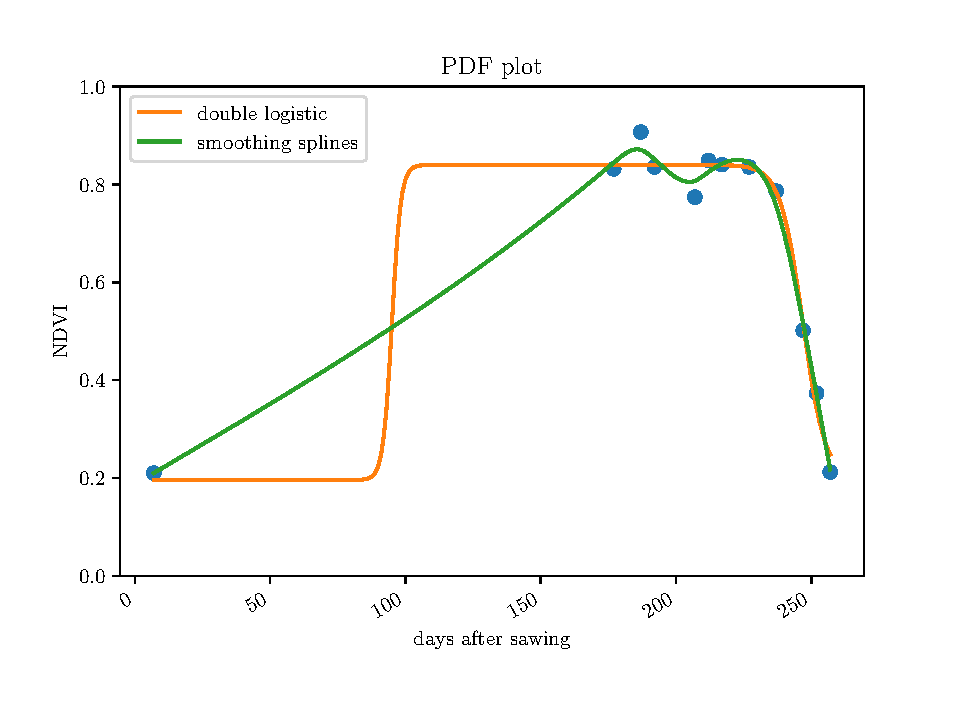
\includegraphics[width=0.5\textwidth]{interpol/test}}
    \end{center}
    \caption{A PGF plot from \texttt{matplotlib}.}
\end{figure}

%%%%%%%%%%%%%%%%%%%%%%%%%%%%%%%%%%%%%%%%%%%%%%%%%%%%%%%%%%%%%

\chapter{Interpolation Methods}

\section{Setting}

We are given data in the form of $\left(x_{i}, Y_{i}\right)$ for $i=1, \ldots, n)$. Assume that it can be represented by
$$
    Y_{i}=m\left(x_{i}\right)+\varepsilon_{i},
$$
where $\varepsilon_i$ is some noise and $m: \mathbb{R} \rightarrow \mathbb{R}$ being some (non-parametric regression) function. If we assume that $\varepsilon_{1}, \ldots, \varepsilon_{n}$ i.i.d. with $\mathbb{E}\left[\varepsilon_{i}\right]=0$ then $$m(x)=\mathbb{E}[Y \mid x]$$
Different assumptions on $m$ will lead to the following models:



\section{Methods - Description}

\subsection{Kernel Regression}
\label{sec:Kernel}
As described previously, we would like to estimate
\begin{equation}
    \label{eq:nadaraya}
    \mathbb{E}[Y \mid X=x]
    = \int_{\mathbb{R}} y f_{Y \mid X}(y \mid x) d y
    =\frac{\int_{\mathbb{R}} y f_{X, Y}(x, y) d y}{f_{X}(x)},
\end{equation}
where $f_{Y \mid X}, f_{X, Y}, f_{X}$ denote the conditional, joint and marginal densities.
This can be done with a kernel $K$:
$$
    \hat{f}_{X}(x)=\frac{\sum_{i=1}^{n} K\left(\frac{x-x_{i}}{h}\right)}{n h}, \hat{f}_{X, Y}(x, y)=\frac{\sum_{i=1}^{n} K\left(\frac{x-x_{i}}{h}\right) K\left(\frac{y-Y_{i}}{h}\right)}{n h^{2}}
$$
By plugging the above into equation \ref{eq:nadaraya} we arrive at the \textit{Nadaraya-Watson} kernel estimator:
$$\hat{m}(x)=\frac{\sum_{i=1}^{n} K\left(\left(x-x_{i}\right) / h\right) Y_{i}}{\sum_{i=1}^{n} K\left(\left(x-x_{i}\right) / h\right)}$$

**Pros**:
- can be assigned degrees of freedom (trace of the hat-matrix)
- estimation of the noise variance $\hat \sigma_\varepsilon^2$ (XXX c.f. CompStat 3.2.2)

**Cons**:
- choice of kernel
- if the $x \mapsto K(x)$ is not continuous, $\hat m $ isn't either
- choice of bandwidth, especially if $x_i$ are not equidistant.

**Examples:**
Normal, Box
For local bandwidth selection see Brockmann et al. (1993) XXX


\subsection{loess}
\label{sec:loess}


\subsection{Savitzky-Golay Filter}
\label{sec:Savitzky–Golay}
The \textit{Savitzky-Golay Filter}, introduced in \cite{savitzkySmoothingDifferentiationData1964} is a technique in signal processing and can be used to filter out high frequencies (low-pass filter) as argued in \cite{schaferWhatSavitzkyGolayFilter2011}. Furthermore, it also can be used for smoothing by filtering high frequency noise while keeping the low frequency signal.
First we choose a window size $m$. Then, for each point $j \in \{m, m+1, \dots, n-m\}$ we fit a polynomial of degree $k$ by:
$$\hat y_j=\min_{p\in P_k}\sum_{i=-m}^{m}(p (x_{j+i})-y_{i+j})^{2},$$
were $P_k$ denotes the Polynomials of degree $k$ over $\mathbb R$.

For equidistant points this can efficiently be calculated by
$$
    \hat y_{j}=\sum_{i=-m}^{m} c_{i} y_{j+i},
$$
where the $c_i$ are only dependent on the $m$ and $k$ and are tabulated in the original paper.

**Pros**
- popular technique in signal processing
- efficient calculation for equidistant points

**Cons**
- no natural way of how to estimate points which are not in the data. XXX

\subsubsection*{Interpolation and Smoothing}
In a rather famous paper \cite{chenSimpleMethodReconstructing2004a} a ``robust'' method based on the Savitzky-Golay has been used.
The method is based on the assumption that due to atmospheric effects the observed NDVI tends to be underestimated and that it cannot increase too quickly\footnote{The latter is argued by the biological impossibility of such fast vegetation changes}.

\textbf{Algorithm:}
\begin{enumerate}
    \item Remove points which are labeled as cloudy
    \item Remove points which would indicate an increase greater than 0.4 within 20 days
    \item Linearly interpolate to obtain an equidistant time series $X^0$
    \item Apply the Savitzky-Golay Filter to obtain a new time series $X^1$
    \item Update $X^1$ by applying again a Savitzky-Golay Filter but this time weight the observations by $w_i = \min\left(1, 1 - \frac{X^1_i-X^0_i}{\max_i\|X^1_i-X^0_i\|}\right)$. This reduces the impact of outliers\footnote{Here we call a point $i$ an outlier if $X^0_i<X^1_i$.} and by repeating this step the authors obtain an ``upper NDVI envelope''
\end{enumerate}

Pros
- Upper envelope matches intuition for the NDVI. Therefore, it is robust against outliers with small values.

Cons
- Not generalizable to other spectral indices.
- Linear interpolation to account for missing data might be not appropriate.
- No smooth interpolation between two measurements.

\subsubsection*{Extension: Spatial-Temporal-Savitzky-Golay Filter}
One notable adaptation of the Savitzky-Golay is the presented by \cite{caoSimpleMethodImprove2018b}. The key difference is the additional assumption of the cloud cover being discontinuous and that we can improve by looking at adjacent pixels\footnote{Here, we say that a pixel is adjacent if it is the same pixel but from a different year (keeping the same day of the year) or (if not enough of such temporal-adjacent pixel are found) it is spatially adjacent}. Because we are working with rather high resolution satellite data, and we need the variance in the predictors we will waive this extension.

\subsection{Double Logistic}
\label{sec:double_logistic}
The Double Logistic smoothing as introduced in \cite{beckImprovedMonitoringVegetation2006} heavily relies on shape assumptions of the fitted curve (i.e. the NDVI time series).

Assumptions:
\begin{itemize}
    \item There is a minimum NDVI level $Y_{\min}$ in the winter (e.g. due to evergreen plants), which might be masked by snow. This can be estimated beforehand, taking into several years into account.
    \item The growth cycle can be divided into an increase and a decrease period where the time series follows a logistic function. The maximum increase (or decrease) is observed at $t_0$ (or $t_1$) with a slope of $d_0$ (or $d_1$).
\end{itemize}

The equation of the double-logistic fit is given by:
\begin{equation*}
    Y(t) = Y_{\min} + \left(Y_{\max}-Y_{\min}\right)\left(\frac{1}{1+e^{-d_0(t-t_0)}}+\frac{1}{1+e^{-d_1(t-t_1)}}-1\right)
\end{equation*}
Where the five free parameters: $Y_{\max}$, $d_0$, $d_1$, $t_0$, $t_1$ are initially estimated by least squares. Similar as for the Savitzky-Golay Filter (c.f. section~\ref{sec:Savitzky–Golay}) we reestimate (only once) the parameters by giving less weight to the overestimated observations and more weight to the underestimated observations\footnote{For the details on the weights we refer to \cite{beckImprovedMonitoringVegetation2006}}.

\subsection{Fourier Approximation}
\label{sec:fourier_approx}
$$
    \operatorname{NDVI}(t)=\sum_{j=0}^{2} a_{j} \times \cos \left(j \times \Phi_{t}\right)+b_{j} \times \sin \left(j \times \Phi_{t}\right)
$$
where $\Phi=2 \pi \times(t-1) / n$.

\cite{beckImprovedMonitoringVegetation2006} shows in their lag-plots a heavy autocorrelation of resiudals



% \subsection{Polynomial interpolation}
% \label{sec:Polynomial}

% \subsection{Polynomial approximation}
% \label{sec:Polynomial}

\subsection{Cubic Smoothing Splines}
\label{sec:Cubic}
We interpolate with a function in $C^2$ (space of three time continuous differentiable functions) which is defined piecewise by cubic polynomials.
**Pros**
Regression splines (B-splines)
\cite{woodSmoothingParameterModel2016}
use a basis of the spline space (e.g. B-splines or j-th cardinal basis) and fit the splines of degree k to approximate the data.

\subsection{B-splines}
\label{sec:B}
from \cite{lycheSplineMethods2005}
$$
    S(x)=\sum_{j=0}^{n-1} c_{j} B_{j, k ; t}(x)
$$
$$
    \begin{array}{r}
        B_{i, 0}(x)=1, \text { if } t_{i} \leq x<t_{i+1}, \text { otherwise } 0 \\
        B_{i, k}(x)=\frac{x-t_{i}}{t_{i+k}-t_{i}} B_{i, k-1}(x)+\frac{t_{i+k+1}-x}{t_{i+k+1}-t_{i+1}} B_{i+1, k-1}(x)
    \end{array}
$$

**Smoothing:**
We can relax the constrain that we have to perfectly interpolate. Thus we use the minimum number of knots\footnote{SciPy uses FITPACK and DFITPACK, the documentation suggests that smoothness is achieved by reducing the number knots used} such that:
$\sum_{i=1}^n(w (y_i - \hat y_i))^2 \leq s$

**Pros**
- can be assigned degrees of freedom
- extendable to "smooth" version
- performs also well if points are not equidistant

**Cons**
- smoothing process does not translate well to a interpretation (unlike smoothing splines)
- choice of smoothing parameter $s$

\subsection{Natural Smoothing Splines}
\label{sec:Natural}
Let $\mathcal F$ be the Sobolev space (the space of functions of which the second derivative is integrable). Then the unique\footnote{Strictly speaking it is only unique for $\lambda > 0$} minimizer
$$\hat m :=\argmin_{f \in \mathcal F} \sum_{i=1}^{n}\left(Y_{i}-{f}\left(x_{i}\right)\right)^{2}+\lambda \int {f}^{\prime \prime}(x)^{2} d x$$
is a natural\footnote{It is called natural since it is affine outside the data range ($\forall x\notin [x_1, x_n]:\hat m''(x) = 0$)} cubic spline.

**Pros:**
- can be assigned degrees of freedom (trace of the hat-matrix)
- efficient estimation (closed form solution)
- intuitive penalty (we don't want the function to be too ``wobbly'' --- change slopes)
- performs also well if points are not equidistant
- fixes the Runge's phenomenon (fluctuation of high degree polynomial interpolation)

**Cons:**
- choose $\lambda$

\subsection{Penalized Regression Splines}
\label{sec:Penalized}
Intuition: similar as Natural Smoothing Splines, but we choose knots

\subsection{Kriging}
\label{sec:Kriging}

Kriging was developed in geostatistics to deal with autocorrelation of the response variable at nearby points. By applying the notion that two spectral indices which are (timewise) close should also take similar values we justify the application of Kriging. In the end we would like to fit a smooth Gaussian process to the data. For this subsection we will follow \cite{diggleGaussianModelsGeostatistical2007}.

\subsubsection*{Definitions and Assumptions}

A \textit{Gaussian Process} $\{S(t) : t\in \mathbb R\} $ is a stochastic process if $(S(t_1),\dots,S(t_k))$ has a multivariate Gaussian distribution for every collection of times ${t_1, \dots , t_k}$.
$S$ can be fully characterized by the mean $\mu(t):=E[S(t)]$ and its covariance function $\gamma\left(t, t^{\prime}\right)=\operatorname{Cov}\left(S(t), S\left(t^{\prime}\right)\right)$

Assumption:
We will assume the Gaussian process to be stationary. That is for $\mu(t)$ to be constant in $t$ and $\gamma(t,t')$ to depend only on $h=t-t'$. Thus, we will write in the following only $\gamma(h)$.\footnote{Note that the process is also \textit{isotropic} (i.e. $\gamma(h)=\gamma(\|h\|$) since we are in a one-dimensional setting and the covariance is symmetric.}


We also define the variogram of a Gaussian process as
$$V(h):=V\left(t, t+h\right):=\frac{1}{2} \operatorname{Var}\left(S(t)-S(t+h)\right)\\ %align XXX
    =(\gamma(0))^2(1-\operatorname{corr}(S(t),S(t+h)))
$$
And decide to use a gaussian Variogram defined by
$$V(h) = p \cdot\left(1-e^{-\frac{h^{2}}{\left(\frac{4}{7} r\right)^{2}}}\right)+n,$$
where $h$ is the distance, $n$ is the nugget, $r$ is the range and $p$ is the partial sill visuilized in figure~\ref{fig:interpol/kriging_gauss_variogram}.\footnote{Strictrly speaking we use a scaled version of the variogram. Thus only the ratio of $p/n$ matters.}
\begin{my_figure}{interpol/kriging_gauss_variogram}
    \caption{Gaussian Variogram with nugget=1, partial sill=3, range=55}
    \label{fig:interpol/kriging_gauss_variogram}
\end{my_figure}

\begin{my_figure}{interpol/kriging_med_vs_ml_param}
\end{my_figure}
\begin{my_figure}{interpol/kriging_effect_of_param}
\end{my_figure}

\subsection{Other Methods to study:}
From inroduction of \cite{chenSimpleMethodReconstructing2004a}:\\
(1) threshold-
based methods, such as the best index slope extraction
algorithm (BISE) (Viovy et al., 1992); (2) Fourier-based
fitting methods (Cihlar, 1996; Roerink et al., 2000; Sellers
et al., 1994); and (3) asymmetric function fitting methods
such as the asymmetric Gaussian function fitting approach
(Jonsson Eklundh, 2002) and the weighted least-squares
linear regression approach (Swets et al., 1999).
